\documentclass[11pt,a4paper]{article}

% ── HAL-friendly preamble ──────────────────────────────────────────
\usepackage[utf8]{inputenc}
\usepackage[T1]{fontenc}
\usepackage[english]{babel}
\usepackage[a4paper,margin=2.5cm]{geometry}
\usepackage{amsmath,amssymb,amsthm}
\usepackage{mathtools}
\usepackage{bm}
\usepackage{graphicx}
\usepackage{booktabs}
\usepackage{array}
\usepackage{caption}
\usepackage{subcaption}
\usepackage{xcolor}
\usepackage{hyperref}
\usepackage{cleveref}

\hypersetup{
  colorlinks=true,
  linkcolor=black,
  citecolor=black,
  urlcolor=blue!50!black,
  pdftitle={HaCI: Harmonic Contour Integration for Edge Detection},
  pdfauthor={Siddharth Basireddy},
}

% Figures live in assets/, one level above this file.
\graphicspath{{../}{./}}

% ── Math shortcuts ──────────────────────────────────────────────────
\newcommand{\R}{\mathbb{R}}
\newcommand{\norm}[1]{\left\lVert#1\right\rVert}
\newcommand{\abs}[1]{\left\lvert#1\right\rvert}
\newcommand{\sgn}{\operatorname{sgn}}
\newcommand{\softplus}{\operatorname{softplus}}
\newcommand{\relu}{\operatorname{ReLU}}

\title{HaCI: Harmonic Contour Integration for Edge Detection}

\author{%
  Siddharth Basireddy%
}

\date{\today}

\begin{document}
\maketitle

\begin{abstract}
This paper describes HaCI (Harmonic Contour Integration), a compact, fully distributed edge detection algorithm. Through the encoding of classical early-visual priors like divisive normalisation, and association-field facilitation and suppression, the algorithm exposes a network made up of a small set of $161$ learnable parameters. The algorithm is composed of four staged operations on an image: the construction of a per-pixel contrast signal and its projection onto circular harmonics (L0), pooling of the harmonics over overlapping cells into von~Mises orientation bins (L1), refinement of the signal via facilitation and suppression (Seed) and the eventual projection of the pooled signal back onto the pixel level (renderer). The renderer back projection is then passed through non-max suppression to retrieve clean edges.
\end{abstract}

\paragraph{Keywords.} Contour Integration, Harmonic Projection, Divisive Normalisation, Filtered Back-Projection, Edge Detection.

% ─────────────────────────────────────────────────────────────────────
\section{Introduction}\label{sec:intro}

One of the primary functions of the early visual cortex is the transformation of retinal input into global contours. As the cortex operates in a highly parallelized fashion, low-level signals are normalized across the visual grid and passed through layers of increasing radius that accumulate evidence across scale. These low-level signals are subjected to cortical transformations such as non-linear saturation~\cite{naka1966srod}, oriented filtering~\cite{hubel1962orientation}, divisive normalization~\cite{heeger1992normalisation,cavanaugh2002surround}, lateral facilitation and inhibition~\cite{kapadia1995dynamics,field1993contour} and figure-ground polarity~\cite{zhou2000border}. At higher levels, contour readouts are sharpened by collinear and co-circular support and normalised against the surrounding activity before being deposited onto a coherent boundary map.

Analogs to the cortical architecture for computer vision require transforming sparse, irregular mechanisms into dense, synchronous operations suitable for array programming models and parallel processing hardware. Deep convolutional and transformer edge detectors have become the dominant approach~\cite{xie2015hed,liu2017rcf,he2019bdcn,pu2022edter,soria2023dexined,ye2024diffusionedge}, recovering contour structure implicitly through millions of learned weights that carry structural priors from the training data alone. The method introduced in this paper revisits older pipelines built from explicit structural priors, like Canny~\cite{canny1986computational} and gPb~\cite{arbelaez2011gpb}, which construct a pixel-level signal and improve it through an interpretable sequence of stages, but hold gain, scale and anisotropy fixed at design time. We deviate from these gradient-based methods, opting for harmonic projection and encoding cortex-like mechanisms as the core heuristic of a compact, fully differentiable four-stage graph, that extracts thin edges from an RGB image while exposing only $161$ learnable scalars to data.

% ─────────────────────────────────────────────────────────────────────
\section{Method}\label{sec:method}

The pipeline operates in four stages; L0, L1, seed and renderer, each with a fixed radius of interaction.

\subsection{L0: Harmonic Projection}\label{sec:l0}

Let $I:\Omega\to\R^3$ be the input image in sRGB, scaled to $[0,1]$; no linearisation is applied. Before L0 the image is reflect-padded at the bottom and right so that the L1 cell grid (\cref{sec:l1}) covers it exactly, and $\Omega$ denotes this padded domain; the boundary map is cropped back to the original image $\Omega_0 \subseteq \Omega$ at the end. The eight-neighbour offsets $\delta_k = (\delta_{y,k}, \delta_{x,k})$, $k = 1, \dots, 8$, in image (row, column) order, have bearings $\phi_k = \operatorname{atan2}(-\delta_{y,k}, \delta_{x,k}) \in \{0, \pi/4, \dots, 7\pi/4\}$, measured anticlockwise from the $+x$ axis with $y$ pointing up (image rows run downwards, hence the sign).
Luminance and chrominance are routed through separate channels of a learned spectral metric, divisively normalised against their own energy and a spatial pool of local contrast, and projected onto circular harmonics to produce per-pixel complex moments $z_1, z_2 \in \mathbb{C}$.

\paragraph{Spectral RGB metric:}
Let $L = (1,1,1)/\sqrt{3}$ be the (fixed) achromatic axis and let $(B_1, B_2)$ be a fixed orthonormal basis of $L^{\perp}$ in $\R^3$. The metric tensor on RGB differences is
\begin{equation}\label{eq:metric}
  M = W^\top W = w_\ell^2\, L L^\top + s_1^2\, b_1 b_1^\top + s_2^2\, b_2 b_2^\top,
\end{equation}
where $(b_1, b_2)$ is the in-plane rotation of $(B_1, B_2)$ by a learned angle $\theta_{\mathrm{chr}}$:
\begin{equation}
  b_1 = \cos\theta_{\mathrm{chr}}\, B_1 + \sin\theta_{\mathrm{chr}}\, B_2,
  \qquad
  b_2 = -\sin\theta_{\mathrm{chr}}\, B_1 + \cos\theta_{\mathrm{chr}}\, B_2.
\end{equation}
The four learned scalars are $(w_\ell, s_1, s_2, \theta_{\mathrm{chr}})$ with $w_\ell, s_1, s_2 \geq 0$ via $\softplus$. Applying the rotation to the basis vectors (rather than as a left multiplier on the row-stack of $W$) is required: the latter would make $\theta_{\mathrm{chr}}$ cancel from $W^\top W$ by orthogonality and become pure gauge. The projected image is $u(p) = W I(p) \in \R^3$, where the rows of $W$ are $w_\ell L$, $s_1 b_1$ and $s_2 b_2$.

\paragraph{JPEG notch:}
Each projected channel $u_j$ is filtered by a learnable separable notch, $\tilde u_j = h_N * u_j$, applied along rows and then columns with replicate padding. The 1D frequency response is real and even,
\begin{equation}\label{eq:notch}
  \hat h_N(\omega) = 1 - d \exp\!\left(-\frac{(\abs{\omega} - \omega_n)^2}{2\sigma_n^2}\right),
\end{equation}
and the kernel of half-width $H_N$ is synthesised from it by a cosine sum over the $L_N = 2H_N + 1$ sampled frequencies $\omega_m = m/L_N$:
\begin{equation}\label{eq:notch-kernel}
  h_N[n] = \frac{1}{L_N}\sum_{m=-H_N}^{H_N} \hat h_N(\omega_m)\cos(2\pi\omega_m n),
  \qquad n \in \{-H_N, \dots, H_N\}.
\end{equation}
The three learnable scalars are $\omega_n = \tfrac{1}{2}\sigma(\cdot) \in (0, \tfrac{1}{2})$ cycles/px, $\sigma_n = \softplus(\cdot)$ and $d = \sigma(\cdot) \in (0, 1)$. They are initialised as a notch at the 8-px JPEG block frequency, $\omega_n = 1/8$, $\sigma_n = 1/32$, $d = 0.8$; the learned response is discussed in \cref{sec:results}.

\paragraph{Directional contrasts:}
For each pixel $p$ and offset $\delta_k$, the squared luminance and chrominance contrasts are taken on the filtered projection,
\begin{equation}\label{eq:dlumchr}
  m_k^{\mathrm{lum}}(p)^2 = \bigl(\tilde u_1(p) - \tilde u_1(p - \delta_k)\bigr)^2,
  \qquad
  m_k^{\mathrm{chr}}(p)^2 = \sum_{j=2}^{3} \bigl(\tilde u_j(p) - \tilde u_j(p - \delta_k)\bigr)^2,
\end{equation}
and set to zero where $p - \delta_k$ falls outside $\Omega$. Without the notch ($\tilde u = u$) these are, by linearity, $w_\ell^2 (L \cdot \Delta c_k)^2$ and $s_1^2 (b_1 \cdot \Delta c_k)^2 + s_2^2 (b_2 \cdot \Delta c_k)^2$ with $\Delta c_k(p) = I(p) - I(p - \delta_k)$: the squared norms of $\Delta c_k$ under the luminance and chrominance blocks of $M$.

\paragraph{Contrast gain control:}
Each channel $\chi \in \{\mathrm{lum}, \mathrm{chr}\}$ is passed through a rational saturating nonlinearity~\cite{naka1966srod} whose denominator also carries the contrast energy pooled over all directions and over a spatial neighbourhood~\cite{heeger1992normalisation}:
\begin{equation}\label{eq:nr}
  h_k^{\chi}(p) = \frac{m_k^{\chi}(p)^2}
                    {\eta_\chi^2 + m_k^{\chi}(p)^2 + \lambda_0\, Q^{\chi}(p)},
  \qquad
  Q^{\chi} = G_{\sigma_r} * \sum_{k'=1}^{8} \bigl(m_{k'}^{\chi}\bigr)^2,
\end{equation}
with $h_k(p) = h_k^{\mathrm{lum}}(p) + h_k^{\mathrm{chr}}(p)$. $G_{\sigma_r}$ is a normalised separable Gaussian truncated at radius $r_Q$ (reflect padding). The pool weight $\lambda_0$ and width $\sigma_r$ are learned through $\softplus$; at $\lambda_0 = 0$, \cref{eq:nr} reduces to a per-direction Naka--Rushton squash. The half-saturation constants $\eta_{\mathrm{lum}}, \eta_{\mathrm{chr}}$ are fixed (\cref{tab:fixed-params}): only $m/\eta$ enters, and the metric gains $w_\ell, s_1, s_2$ already set that scale.

\paragraph{Harmonic projection:}
The eight values $\{h_k(p)\}_{k=1}^{8}$ are projected onto the first two circular harmonics, yielding a complex dipole $z_1$ (polarity) and quadrupole $z_2$ (orientation, double-angle):
\begin{equation}\label{eq:zn}
  \boxed{\;
  z_n(p) = \sum_{k=1}^{8} h_k(p)\, e^{i n \phi_k},
  \qquad n \in \{1, 2\}.\;}
\end{equation}
The second-harmonic magnitude $h_{2m}(p) = \abs{z_2(p)}$ is exported separately. Image-border pixels (for which $\delta_k$ would step outside $\Omega$) are zeroed. Only $z_2$ is used downstream; $z_1$ is exported for diagnostics. Because $h_k$ is largest for offsets that cross an edge, $\theta_p = \tfrac{1}{2}\arg z_2(p)$ is the angle of the edge normal in the $y$-up frame. In image $(y, x)$ order the normal is $(-\sin\theta_p, \cos\theta_p)$ and the tangent is $(\cos\theta_p, \sin\theta_p)$; all orientations below follow this convention.

\subsection{L1: Cell-Level Orientation Binning}\label{sec:l1}

The padded image (\cref{sec:l0}) is partitioned into overlapping $P{\times}P$ cells with stride $D = P - O$, indexed by $c$. Because $D < P$, a cell shares pixels with every cell up to $\lfloor (P - 1)/D \rfloor = 2$ steps away in each direction, $24$ neighbours in all. Inside cell $c$ with pixel set $\mathcal{P}_c$, the per-pixel orientation estimate is $\theta_p = \tfrac{1}{2}\arg z_2(p)$. With $K$ orientation bins of centres $\bar\theta_k = k\pi/K$ for $k=0,\dots,K-1$, the per-pixel von~Mises weight is
\begin{equation}\label{eq:vm-weight}
  v_k(\theta_p) = \exp\!\bigl(\kappa_{\mathrm{vm}}\,(\cos(2(\theta_p - \bar\theta_k)) - 1)\bigr),
\end{equation}
with learnable concentration $\kappa_{\mathrm{vm}} > 0$ ($\softplus$). The per-bin energy and sub-pixel anchors are
\begin{equation}\label{eq:rho-bin}
  \boxed{\;
  \rho^{(k)}(c) = \sum_{p \in \mathcal{P}_c} \abs{z_2(p)}\, v_k(\theta_p)\, \mathrm{ok}_p,\;}
\end{equation}
\begin{equation}\label{eq:anchor-bin}
  a_x^{(k)}(c) = \frac{\sum_{p} \abs{z_2(p)}\, v_k(\theta_p)\, x_p\, \mathrm{ok}_p}{\sum_{p} \abs{z_2(p)}\, v_k(\theta_p)\, \mathrm{ok}_p + \varepsilon},
\end{equation}
and similarly $a_y^{(k)}(c)$, where $\mathrm{ok}_p \in \{0,1\}$ excludes border pixels. Cells whose border-pixel fraction exceeds $0.2$, or that extend past the unpadded image, are flagged as $\mathrm{ok}(c) = 0$: the seed sets their response to zero and the renderer deposits nothing from them. They still count as neighbours: the seed's facilitation, surround and flank means (\cref{sec:seed}) are normalised by fixed kernel sums, so a flagged cell enters them with value zero.

The output of L1 is the per-bin tensor $\rho^{(k)}(c) \in \R^{N \times K}$ together with the sub-pixel anchors $(a_x^{(k)}, a_y^{(k)})$ and the bin centres $\bar\theta_k$. L1 has no learned parameters of its own; $\kappa_{\mathrm{vm}}$ is stored with the seed's parameters, and L1 is recomputed at every training step from the live L0 output, so gradients reach $\kappa_{\mathrm{vm}}$ through the bin weights $v_k$.

\subsection{Seed: Gain Control}\label{sec:seed}

The seed refines the L1 signal, converting the per-bin energies $\rho^{(k)}$ into a per-bin readout $\rho_{\mathrm{out}}^{(k)}(c) \in [0, 1]$, from which a per-cell scalar $\rho(c)$ and an orientation $\theta(c)$ are read. Each bin is facilitated by a co-circular association field along its tangent and divisively normalised against the same orientation in the surrounding cells and in the cells that flank it along its normal.

The per-cell state the seed produces (a boundary strength $\rho(c)$, an orientation $\theta(c)$, and a sub-pixel anchor) is designed to be task-agnostic: a mid-level contour representation that downstream stages could consume directly for segmentation, grouping, or shape analysis. We use the term \emph{seed} in this sense, as the distilled contour signal from which further processing proceeds. For the edge-detection task treated here that further processing is a single stage: the renderer (\cref{sec:render}) back-projects the seed onto the pixel grid. The seed's architecture does not depend on this choice of readout, but its parameters do: they are trained only through the renderer and the edge loss, and the per-cell exports are not on that path (see the cell-level export below), so their use as a general representation is untested here.

\paragraph{Per-bin Naka--Rushton squash:}
With $R^{(k)}(c) = \rho^{(k)}(c)\,\mathrm{ok}(c)$ and learnable half-saturation $\eta_z > 0$,
\begin{equation}\label{eq:rho-nr}
  \rho_{\mathrm{NR}}^{(k)}(c) = \frac{R^{(k)}(c)^2}{R^{(k)}(c)^2 + \eta_z^2 + \varepsilon}\,\mathrm{ok}(c).
\end{equation}

\paragraph{Co-circular association field:}
For bin $k$ let $\hat t_k = (\cos\bar\theta_k, \sin\bar\theta_k)$ and $\hat n_k = (-\sin\bar\theta_k, \cos\bar\theta_k)$ be the tangent and normal in $(dy, dx)$ order. A cell offset $\delta \neq 0$ in the square neighbourhood $\mathcal{N}_f$ of radius $r_f$ has tangent and normal coordinates $t_k(\delta) = \delta \cdot \hat t_k$ and $n_k(\delta) = \delta \cdot \hat n_k$, and makes the angle $\psi_k(\delta) = \arctan\bigl(n_k(\delta)/t_k(\delta)\bigr) \in (-\pi/2, \pi/2)$ with the tangent axis. Its weight
\begin{equation}\label{eq:pos-t}
  w_k(\delta) = \exp\!\left(-\frac{\norm{\delta}^2}{2\sigma_f^2}\right)
                \exp\!\bigl(\kappa_a \bigl(\cos 2\psi_k(\delta) - 1\bigr)\bigr),
  \qquad
  \cos 2\psi_k(\delta) = \frac{t_k(\delta)^2 - n_k(\delta)^2}{\norm{\delta}^2},
\end{equation}
separates reach ($\sigma_f$) from direction tuning ($\kappa_a$).

The neighbour at $\delta$ lies on the circle tangent to $\bar\theta_k$ at $c$ with curvature $\kappa_k(\delta) = 2\abs{n_k(\delta)}/\norm{\delta}^2$, and the circle's tangent at $c + \delta$ is turned by $2\psi_k(\delta)$~\cite{parent1989trace}. Bin $k$ reads the neighbour at the fractional bin position
\begin{equation}\label{eq:cocirc-read}
  q_k(\delta) = k + s_k(\delta)\, \frac{2\psi_k(\delta)\, K}{\pi},
  \qquad
  s_k(\delta) = \frac{\sigma_\kappa^2}{\sigma_\kappa^2 + \kappa_k(\delta)^2},
\end{equation}
linearly interpolated between the two nearest bins (bin indices modulo $K$, $\{q\} = q - \lfloor q \rfloor$):
\begin{equation}\label{eq:cocirc-interp}
  \tilde\rho^{(k)}_{\delta}(c) = \bigl(1 - \{q_k(\delta)\}\bigr)\, \rho_{\mathrm{NR}}^{(\lfloor q_k(\delta) \rfloor)}(c + \delta)
                               + \{q_k(\delta)\}\, \rho_{\mathrm{NR}}^{(\lfloor q_k(\delta) \rfloor + 1)}(c + \delta).
\end{equation}
Turns implied by curvatures within the learned tolerance $\sigma_\kappa$ (in 1/cell) are expected; sharper ones are read as straight continuation. At $\sigma_\kappa = 0$ the read is the same-bin collinear one.

Support is collected separately ahead of and behind the cell, each lobe normalised by its own weight,
\begin{equation}\label{eq:lobes}
  f_{\pm}^{(k)}(c) = \frac{\sum_{\delta \in \mathcal{N}_f,\ \pm t_k(\delta) > 0} w_k(\delta)\, \tilde\rho^{(k)}_{\delta}(c)}
                          {\sum_{\delta \in \mathcal{N}_f,\ \pm t_k(\delta) > 0} w_k(\delta) + \varepsilon},
\end{equation}
so a cell inside a long contour sees $f_+ \approx f_- \approx$ the contour's response; offsets with $t_k(\delta) = 0$ belong to neither lobe. The lobes give the mean association support and a gap bridge, their harmonic mean:
\begin{equation}\label{eq:rho-assoc}
  \rho_{\mathrm{assoc}}^{(k)}(c) = \tfrac{1}{2}\bigl(f_+^{(k)}(c) + f_-^{(k)}(c)\bigr),
  \qquad
  b^{(k)}(c) = \frac{2\, f_+^{(k)}(c)\, f_-^{(k)}(c)}{f_+^{(k)}(c) + f_-^{(k)}(c) + \varepsilon}.
\end{equation}
The interpolation weights sum to one over the input bins, so each lobe in \cref{eq:lobes} stays a weighted mean of the neighbours' responses and its normaliser needs only the spatial weights $w_k$. The field is a bank of $2K \times K$ kernels of size $(2r_f + 1)^2$, built from $(\sigma_f, \kappa_a, \sigma_\kappa)$ and applied as a single convolution with reflect padding.

\paragraph{Same-orientation Surround:}
Each bin is pooled over the neighbouring cells of the same bin with a Gaussian of width $\sigma_S$ over the square neighbourhood $\mathcal{N}_S$ of radius $r_S$, the cell itself excluded:
\begin{equation}\label{eq:S}
  S^{(k)}(c) = \frac{\sum_{\delta \in \mathcal{N}_S \setminus \{0\}} G_{\sigma_S}(\delta)\, \rho_{\mathrm{NR}}^{(k)}(c + \delta)}
                    {\sum_{\delta \in \mathcal{N}_S \setminus \{0\}} G_{\sigma_S}(\delta)},
  \qquad
  G_{\sigma_S}(\delta) = \exp\!\left(-\frac{\norm{\delta}^2}{2\sigma_S^2}\right).
\end{equation}
Each bin's pool reads only that bin, so the pool has no cross-orientation terms: its orientation tuning is the bin tuning set by $\kappa_{\mathrm{vm}}$, and the readout codes each cell relative to its same-orientation context. Only the cell is excluded, not its pixels: the $24$ nearest cells overlap it (\cref{sec:l1}), so $S$ also reads part of the cell's own L1 input and acts as a near-field same-orientation pool rather than a surround outside the cell's footprint. The near offsets of the association field overlap the cell in the same way; \cref{sec:results} gives the weight shares in the released model. $G_{\sigma_S}$ is separable: it is applied as a depthwise row and column convolution (reflect padding) and the centre tap is subtracted.

\paragraph{Flank Suppression:}
$S$ is isotropic, so it cannot tell a contour with parallel neighbours on both sides, as in texture and gratings, from one that runs alone. A second same-bin pool reads the cells on either side of $c$ along the bin normal. Over the square neighbourhood $\mathcal{N}_{\mathrm{fl}}$ of radius $r_{\mathrm{fl}}$, an offset $\delta$ is weighted by
\begin{equation}\label{eq:flank-w}
  u_k(\delta) = \exp\!\left(-\frac{\norm{\delta}^2}{2\sigma_{\mathrm{fl}}^2}\right)
                \exp\!\bigl(\kappa_{\mathrm{fl}} \bigl(\cos 2\psi^{\perp}_k(\delta) - 1\bigr)\bigr),
  \qquad
  \cos 2\psi^{\perp}_k(\delta) = \frac{n_k(\delta)^2 - t_k(\delta)^2}{\norm{\delta}^2},
\end{equation}
where $\psi^{\perp}_k(\delta)$ is the angle between $\delta$ and the normal $\hat n_k$, with $t_k, n_k$ as in \cref{eq:pos-t}. Offsets within Chebyshev distance $r_{\mathrm{ex}} = \lceil P/D \rceil - 1 = 2$ are left out. These are the $24$ cells that share pixels with $c$ (\cref{sec:l1}); a lone edge spreads into them, so without the exclusion it would flank itself. The two sides are normalised separately, like the association lobes:
\begin{equation}\label{eq:flank-sides}
  U_{\pm}^{(k)}(c) = \frac{\sum_{\delta \in \mathcal{N}_{\mathrm{fl}}^{\pm}} u_k(\delta)\, \rho_{\mathrm{NR}}^{(k)}(c + \delta)}
                          {\sum_{\delta \in \mathcal{N}_{\mathrm{fl}}^{\pm}} u_k(\delta) + \varepsilon},
  \qquad
  \mathcal{N}_{\mathrm{fl}}^{\pm} = \bigl\{\delta \in \mathcal{N}_{\mathrm{fl}} : \norm{\delta}_\infty > r_{\mathrm{ex}},\ \pm n_k(\delta) > 0\bigr\}.
\end{equation}
They are combined by their harmonic mean,
\begin{equation}\label{eq:flank}
  U^{(k)}(c) = \frac{2\, U_+^{(k)}(c)\, U_-^{(k)}(c)}{U_+^{(k)}(c) + U_-^{(k)}(c) + \varepsilon},
\end{equation}
which, like the gap bridge of \cref{eq:rho-assoc}, is non-zero only when both sides are occupied. Gratings and texture, with parallel structure on both sides, are suppressed; a lone edge, or an edge beside a single parallel one, is not. Each bin reads only its own channel, so the flank pool is a bank of $2K$ kernels of size $(2r_{\mathrm{fl}} + 1)^2$, built from $\sigma_{\mathrm{fl}}$ and applied as a grouped convolution with reflect padding. The normal tuning $\kappa_{\mathrm{fl}}$ is fixed.

\paragraph{Divisive Readout:}
Association support scales the cell's own response, and the bridge adds a term that is non-zero only where there is support on both sides:
\begin{equation}\label{eq:e}
  e^{(k)}(c) = \rho_{\mathrm{NR}}^{(k)}(c)\,\bigl(\beta_{\mathrm{seed}} + \beta_{\mathrm{assoc}}\, \rho_{\mathrm{assoc}}^{(k)}(c)\bigr) + \beta_{\mathrm{gap}}\, b^{(k)}(c).
\end{equation}
Because the facilitation is multiplicative it cannot create a response past a line end, and the bridge fills gaps without extending ends. The excitation is divisively normalised against the surround and the flanks through a Michaelis--Menten-style readout~\cite{naka1966srod,heeger1992normalisation}:
\begin{equation}\label{eq:rho-out-bin}
  \boxed{\;
  \rho_{\mathrm{out}}^{(k)}(c) = \frac{\bigl(e^{(k)}(c)\bigr)^2}
                                       {\bigl(e^{(k)}(c)\bigr)^2 + \eta_r^2 + \lambda\, \bigl(S^{(k)}(c)\bigr)^2 + \lambda_{\mathrm{fl}}\, \bigl(U^{(k)}(c)\bigr)^2 + \varepsilon},\;}
\end{equation}
with learnable gains $(\beta_{\mathrm{seed}}, \beta_{\mathrm{assoc}}, \beta_{\mathrm{gap}})$, readout half-saturation $\eta_r$, surround weight $\lambda$ and flank weight $\lambda_{\mathrm{fl}}$, all positive via $\softplus$. The squared $e$ on numerator and denominator gives a Naka--Rushton-shaped transfer with bounded range. $\lambda S^2$ raises the half-saturation point where the neighbouring cells carry the same orientation, and $\lambda_{\mathrm{fl}} U^2$ raises it further where parallel contours occupy both flanks.

\paragraph{Cell-level Export:}
Three quantities are exported per cell. The scalar boundary strength $\rho(c) \in [0, 1]$ is the maximum over bins, returned through a straight-through estimator so the forward pass is hard while the backward pass is smooth:
\begin{equation}\label{eq:rho-cell}
  \rho(c) = \max_k \rho_{\mathrm{out}}^{(k)}(c),
  \qquad
  \tilde\rho(c) = \sum_k \mathrm{softmax}_\tau\!\bigl(\rho_{\mathrm{out}}^{(\cdot)}(c)\bigr)_k\, \rho_{\mathrm{out}}^{(k)}(c),
\end{equation}
with the standard STE construction $\rho(c) - \tilde\rho(c)_{\mathrm{detach}} + \tilde\rho(c)$ on the forward graph (temperature $\tau$ fixed). The cell orientation is a double-angle weighted blend across bins,
\begin{equation}\label{eq:theta-cell}
  \theta(c) = \tfrac{1}{2}\operatorname{atan2}\!\Bigl(
    \sum_k \rho_{\mathrm{out}}^{(k)}(c)\, \sin 2\bar\theta_k,\;
    \sum_k \rho_{\mathrm{out}}^{(k)}(c)\, \cos 2\bar\theta_k + \varepsilon\Bigr),
\end{equation}
and the cell anchor is taken at the dominant bin $k^\star(c) = \arg\max_k \rho_{\mathrm{out}}^{(k)}(c)$:
\begin{equation}\label{eq:anchor-cell}
  \bigl(a_x^\star(c),\, a_y^\star(c)\bigr) = \bigl(a_x^{(k^\star)}(c),\, a_y^{(k^\star)}(c)\bigr).
\end{equation}
The renderer consumes the full per-bin tensor $\rho_{\mathrm{out}}^{(k)} \in \R^{N\times K}$, the per-bin anchors $(a_x^{(k)}, a_y^{(k)})$ and the bin centres $\bar\theta_k$, not $\rho(c)$, so that it can deposit each bin separately and aggregate with a noisy-OR. The cell-level quantities $\rho(c)$, $\theta(c)$ and $a^\star(c)$ are exports of the mid-level representation and are not on the training-loss path; in particular the STE temperature $\tau$ does not affect training.

\subsection{Renderer: Ramp-filtered Back-projection}\label{sec:render}

The renderer deposits each active (cell, bin) pair onto the pixel grid as a thin curved stroke shaped by two learned 1D kernels, then aggregates contributions via a noisy-OR. The construction borrows the geometry of filtered back-projection~\cite{kak2001ct}; each pair contributes mass along an oriented line through its anchor, and the radial filter is constrained to the windowed-ramp inverse-Radon family. This is not a filtered back-projection in the analytic sense: L0+L1 produce a local orientation-energy field rather than line integrals, the longitudinal profile $h_\parallel$ is a learned finite-support stroke rather than a ray delta, and aggregation across pairs is multiplicative (noisy-OR) rather than additive. The renderer thus exploits FBP's back-projection topology while leaving the inversion identity behind.

\paragraph{Per-bin Features and Correction MLP:}
For each (cell, bin) pair a 5-dimensional feature vector is computed from $\rho_{\mathrm{out}}^{(k)}$ and its $3{\times}3$ neighbourhood:
\begin{equation}\label{eq:feats}
  F^{(k)}_c = \bigl[\, \rho_{\mathrm{out}}^{(k)}(c),\; \mu^{(k)}_{\mathrm{coll}}(c),\; \mu^{(k)}_{t}(c),\; \textstyle\sum_{j \neq k} \rho_{\mathrm{out}}^{(j)}(c),\; \mu^{(k)}_{n}(c)\,\bigr] \in \R^5,
\end{equation}
where $\mu^{(k)}_{\mathrm{coll}}$ is a position-weighted collinear support, and $\mu^{(k)}_{t}, \mu^{(k)}_{n}$ are signed tangent and normal asymmetries of $\rho_{\mathrm{out}}^{(k)}$ across the $3{\times}3$ neighbourhood (concrete definitions in \cref{app:feats}). The features are computed on a detached copy of $\rho_{\mathrm{out}}$, with zeros outside the cell grid and at border cells. A small shared MLP $\Phi : \R^5 \to \R^4$ with one hidden layer of width $12$ emits four raw outputs which are bounded by tanh and softplus:
\begin{equation}\label{eq:mlp-bounded}
  \begin{aligned}
    \kappa^{(k)}_c       &= \kappa_{\max}\, \tanh\!\bigl(\Phi_1(F^{(k)}_c)\bigr), \\
    \xi^{(k)}_c          &= \xi_{\max}\, \tanh\!\bigl(\Phi_2(F^{(k)}_c)\bigr), \\
    \delta_{n}{}^{(k)}_c &= \delta_{n,\max}\, \tanh\!\bigl(\Phi_3(F^{(k)}_c)\bigr), \\
    \alpha^{(k)}_c       &= \exp\!\bigl(\alpha_{\mathrm{range}}\, \tanh\!\bigl(\Phi_4(F^{(k)}_c)\bigr)\bigr),
  \end{aligned}
\end{equation}
where $\kappa_{\max}, \xi_{\max}, \delta_{n,\max}, \alpha_{\mathrm{range}}$ are learnable positive bounds. The four scalars are a curvature, a tangent-direction shift of the stroke vertex, a normal-direction anchor correction, and a multiplicative amplitude $\alpha \in [e^{-\alpha_{\mathrm{range}}}, e^{+\alpha_{\mathrm{range}}}]$. At initialisation $\Phi$ outputs nearly zero, so $\kappa, \xi, \delta_n \approx 0$ and $\alpha \approx 1$, recovering an unmodulated straight stroke.

\paragraph{Sparsity Gate:}
Each cell's bins compete via a winner-decay gate
\begin{equation}\label{eq:gate}
  g^{(k)}(c) = \exp\!\left(\frac{\rho_{\mathrm{out}}^{(k)}(c) - \max_j \rho_{\mathrm{out}}^{(j)}(c)}{T_{\mathrm{gate}}}\right)\, \mathrm{ok}(c),
\end{equation}
with learnable temperature $T_{\mathrm{gate}} > 0$. The dominant bin always satisfies $g = 1$; lagging bins decay exponentially in the $\rho$-gap. Co-equal maxima (junctions) both fire at full gain. Pairs with $g < 10^{-3}$ or $\rho_{\mathrm{out}}^{(k)} < 10^{-4}$ contribute nothing. On CPU and CUDA they are dropped from the active set, so the MLP and synthesis run only on surviving pairs; on Apple GPUs (MPS) every pair is kept with zero amplitude, so that tensor shapes depend only on the image size. Both give the same map.

\paragraph{Anchor correction.}
The bin anchor $(a_x^{(k)}, a_y^{(k)})$ from \cref{eq:anchor-bin} is shifted along the bin normal by $\delta_n$:
\begin{equation}\label{eq:anchor-shift}
  \tilde a^{(k)}_c = \bigl(a_x^{(k)}(c) + \delta_{n}{}^{(k)}_c \cos\bar\theta_k,\;
                            a_y^{(k)}(c) - \delta_{n}{}^{(k)}_c \sin\bar\theta_k\bigr).
\end{equation}

\paragraph{Curved Stroke Synthesis:}
For each pixel $p$ in the deposit window of $\tilde a^{(k)}_c$, let $\Delta = p - \tilde a^{(k)}_c$. Project onto the bin tangent and normal,
\begin{equation}\label{eq:proj}
  s = \Delta_y \cos\bar\theta_k + \Delta_x \sin\bar\theta_k,
  \qquad
  n = -\Delta_y \sin\bar\theta_k + \Delta_x \cos\bar\theta_k,
\end{equation}
shift the tangent coordinate by $\xi$ and bend the normal coordinate by the parabolic curvature term,
\begin{equation}\label{eq:bend}
  \tilde s = s - \xi^{(k)}_c, \qquad n_c = n - \tfrac{1}{2}\kappa^{(k)}_c\, \tilde s^{2},
\end{equation}
and synthesise the (non-negative) stroke profile by a product of learned 1D kernels:
\begin{equation}\label{eq:f}
  f^{(k)}_c(p) = \relu\!\bigl(h_{\perp}(n_c)\, h_{\parallel}(\tilde s)\bigr).
\end{equation}
Both kernels are evaluated at continuous query positions by linear interpolation between integer taps.

\paragraph{Learned 1D Kernels:}
The radial filter $h_{\perp}$ is parameterised as a windowed ramp from the inverse-Radon family,
\begin{equation}\label{eq:h-perp}
  h_{\perp}[n] = \mathrm{IFFT}\bigl(\abs{\omega}\, \mathcal{W}(\omega)\bigr)[n],
  \qquad n \in \{-H_w, \dots, H_w\},
\end{equation}
where $\mathcal{W}(\omega) \geq 0$ is a monotonically decreasing window in $\abs{\omega}$, parameterised by $H_w + 1$ logits $(\nu_0, \dots, \nu_{H_w})$ via
$\mathcal{W}(0) = \softplus(\nu_0)$, $\mathcal{W}(\omega_{m+1}) = \mathcal{W}(\omega_m)\,\sigma(\nu_{m+1})$.
This constrains $h_{\perp}$ to the shape of an FBP ramp filter and initialises it to a Hann window of cutoff $\omega_c$; the resulting profile is the FBP-shaped piece of the renderer.

The longitudinal profile $h_{\parallel}$ is an even, monotonically decreasing function from a positive peak, parameterised by $H_w$ decay-ratio logits $(\zeta_1, \dots, \zeta_{H_w})$ and one peak parameter $h_0$:
\begin{equation}\label{eq:h-par}
  h_{\parallel}[m] = h_0 \prod_{j=1}^{\abs{m}} \sigma(\zeta_j),
  \qquad h_0 = \softplus(h_{0,\mathrm{raw}}),
\end{equation}
initialised to a Gaussian of width $\sigma_{\parallel,0}$.

\paragraph{Per-pair Claim and Noisy-OR Aggregation:}
The per-pair pixel claim is
\begin{equation}\label{eq:claim}
  \mathrm{claim}^{(k)}_c(p) = \alpha^{(k)}_c\, g^{(k)}(c)\, \rho_{\mathrm{out}}^{(k)}(c)\, f^{(k)}_c(p),
\end{equation}
clamped into $[0, 1-\epsilon_c]$ for numerical stability, and the global boundary map is the noisy-OR over all active pairs:
\begin{equation}\label{eq:noisy-or}
  \boxed{\;
  \hat B(p) = 1 - \prod_{(c, k)\in\mathcal{A}} \bigl(1 - \mathrm{claim}^{(k)}_c(p)\bigr).\;}
\end{equation}
In log space, $\log(1 - \hat B(p)) = \sum_{(c, k)} \log(1 - \mathrm{claim}^{(k)}_c(p))$, which is computed by scatter-add on the pixel-flat index and stably back-propagates through both the synthesis and the learned kernels. The anchors and the MLP features are treated as constants in the backward pass, so the renderer passes gradient to the seed and earlier stages only through $\rho_{\mathrm{out}}^{(k)}$, in the claim and in the gate.

\paragraph{Inference:}
At inference, $\hat B$ is thinned by ridge non-maximum suppression along the claim-weighted dominant orientation $\theta^\star(p)$ (the circular mean of $\bar\theta_k$ weighted by per-pair claims): a pixel is kept if it is no smaller than its bilinearly sampled neighbours one pixel either way along the normal. The thinned map is thresholded at $t_{\mathrm{edge}} = 1/2$; for benchmarking the threshold is swept instead (\cref{sec:results}).

% ─────────────────────────────────────────────────────────────────────
\section{Training}\label{sec:train}

The loss is HED-style class-balanced binary cross-entropy~\cite{xie2015hed}. Let $y(p) \in [0, 1]$ be the ground-truth target and $\hat B(p)$ the prediction, clamped to $[10^{-6}, 1 - 10^{-6}]$. The loss is taken over the original image $\Omega_0$, which has $n_+$ positive pixels ($y(p) \geq \tfrac{1}{2}$) and $n_- = \abs{\Omega_0} - n_+$ negative ones:
\begin{equation}\label{eq:loss}
  \mathcal{L} = -\frac{1}{\abs{\Omega_0}}\sum_{p \in \Omega_0}\Bigl[\frac{n_-}{\abs{\Omega_0}}\, y(p)\log\hat B(p) + \frac{n_+}{\abs{\Omega_0}}\,(1 - y(p))\log(1 - \hat B(p))\Bigr],
\end{equation}
computed per image and averaged over the batch.
Gradients flow through all four stages: through the renderer's MLP, correction bounds, gate temperature and 1D kernels; through the seed's thirteen scalars; through the L1 von~Mises weights via $\kappa_{\mathrm{vm}}$; and through the L0 metric $(w_\ell, s_1, s_2, \theta_{\mathrm{chr}})$, notch $(\omega_n, \sigma_n, d)$ and gain control $(\lambda_0, \sigma_r)$. Because every L0 parameter is learned, L0 and L1 are recomputed at every step; the training cache holds only the padded RGB image, the ground truth and the border mask.

We train on the 300-image BRIND train split~\cite{pu2021rindnet}\footnote{\url{https://github.com/xavysp/BRIND}}, the BSDS500 images~\cite{arbelaez2011gpb} re-annotated for reflectance, illumination, normal and depth discontinuities and merged into one edge map per image. We use Adam~\cite{kingma2014adam} with a learning rate of $5\times 10^{-2}$ annealed on a cosine schedule to $5\times 10^{-3}$, gradient clipping at $\norm{\nabla}_2 \leq 1$, batch size $4$, for $50$ epochs.

% ─────────────────────────────────────────────────────────────────────
\section{Results}\label{sec:results}

\Cref{tab:brind} reports the released model on the 200-image BRIND test set. Evaluation follows the Berkeley boundary benchmark~\cite{arbelaez2011gpb}: at each of $99$ thresholds the prediction is binarised, thinned to one-pixel width and matched one-to-one against the ground truth within $0.0075$ of the image diagonal ($\approx 4.3$\,px on $481 \times 321$ images). ODS is the F-measure at the best dataset-wide threshold, OIS the F-measure of the match counts pooled with each image at its own best threshold, and AP the area under the precision--recall curve. Two outputs are scored: the ridge-NMS map of \cref{sec:render} and the soft map $\hat B$.

\begin{table}[h]
\centering
\caption{BRIND test set (200 images), trained on the 300-image BRIND train split. Precision and recall are taken at the ODS threshold ($0.71$ for both maps).}
\label{tab:brind}
\renewcommand{\arraystretch}{1.15}
\begin{tabular}{lccccc}
\toprule
Output & ODS & Precision & Recall & OIS & AP \\
\midrule
Ridge-NMS map & $0.7179$ & $0.6791$ & $0.7614$ & $0.7402$ & $0.7651$ \\
Soft map $\hat B$ & $0.7158$ & $0.6842$ & $0.7505$ & $0.7373$ & $0.6723$ \\
\bottomrule
\end{tabular}
\end{table}

Four learned properties change how the corresponding stages should be read. The notch moved away from its JPEG initialisation to $\omega_n = 0.41$, $\sigma_n = 0.20$, $d = 0.68$; at the five sampled frequencies $0, 1/9, \dots, 4/9$ cycles/px its gain is $0.91, 0.77, 0.56, 0.37, 0.33$, so it acts as a broad high-frequency cut rather than a notch. The curvature tolerance fell to $\sigma_\kappa = 0.007$, which shifts the co-circular read of \cref{eq:cocirc-read} by at most $0.04$ of a bin: in the released model the association field is effectively collinear. The surround and the association field settled at different reaches. With $\sigma_S = 1.69$ cells, $74\%$ of the surround weight falls on the $24$ cells that share pixels with the cell, so $S$ stays a near-field pool. The association reach grew to $\sigma_f = 3.33$ cells, which leaves only $31$--$41\%$ of each facilitation lobe's weight, depending on the bin, on those cells. Finally, the flank weight grew from its near-zero initialisation ($0.01$) to $\lambda_{\mathrm{fl}} = 5.20$. With $\sigma_{\mathrm{fl}} = 1.48$ cells, $79$--$83\%$ of each flank's weight falls on the ring at Chebyshev distance $3$, the nearest cells that share no pixels with the centre cell.

% ─────────────────────────────────────────────────────────────────────
\section{Qualitative Example}\label{sec:qualitative}

HaCI applied to a single natural image is shown in \cref{fig:example}. The input (\cref{fig:base}) is a $1280 \times 961$ full-colour photograph of zebras on dry grassland, from outside the BRIND splits, with luminance and chrominance contrasts that L0 routes through the learned spectral metric. The output (\cref{fig:edges}) is the inference output of \cref{sec:render}: $\hat B$ thinned by ridge non-maximum suppression along the claim-weighted orientation $\theta^\star(p)$ and thresholded at $t_{\mathrm{edge}} = 1/2$. White pixels mark the surviving one-pixel-wide contours.

\begin{figure}[t]
  \centering
  \begin{subfigure}[t]{0.48\textwidth}
    \vspace{0pt}
    \centering
    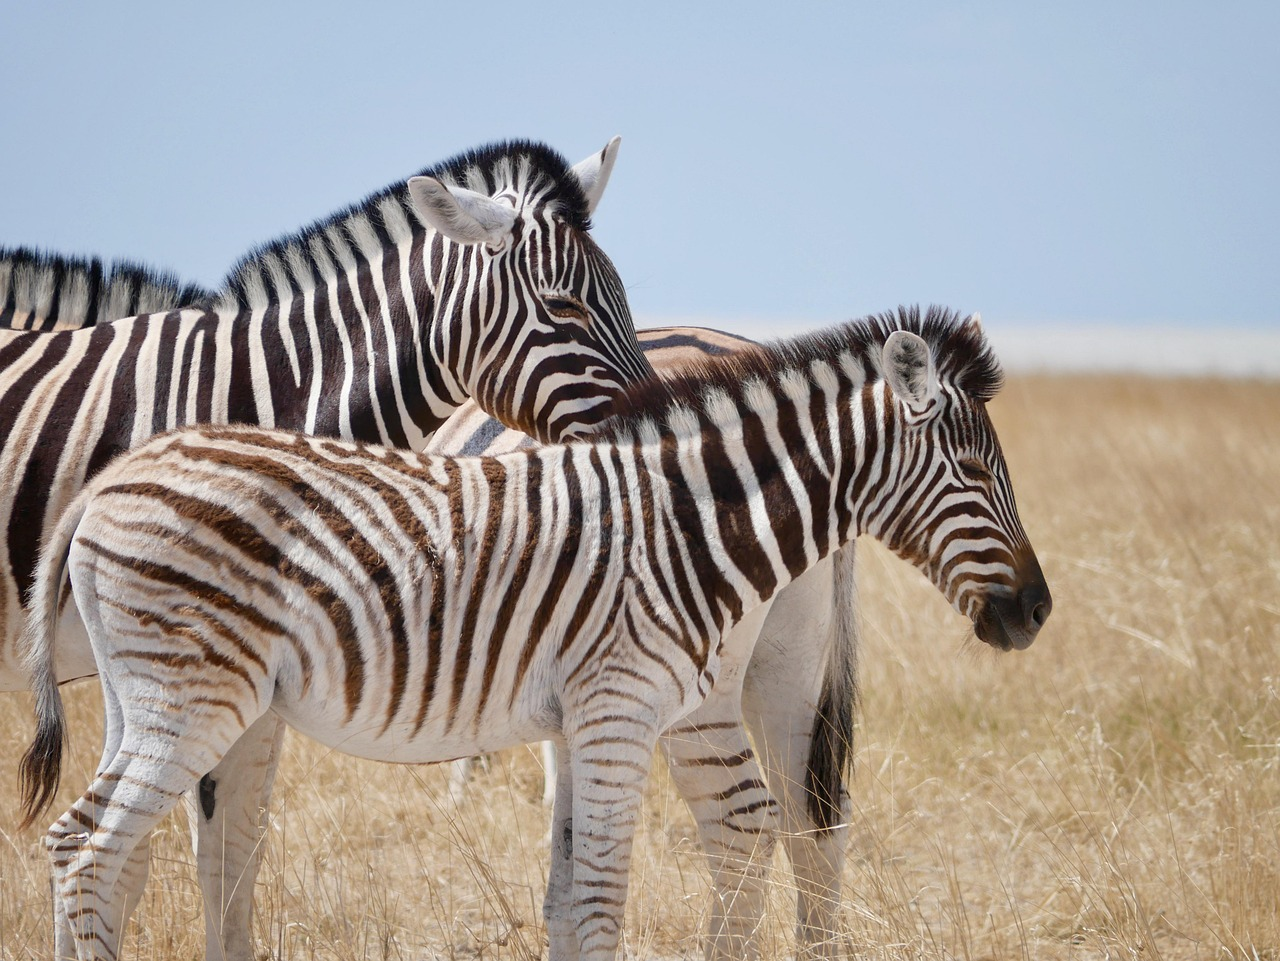
\includegraphics[width=\linewidth]{base.png}
    \caption{Input image $I$.}
    \label{fig:base}
  \end{subfigure}%
  \hfill
  \begin{subfigure}[t]{0.48\textwidth}
    \vspace{0pt}
    \centering
    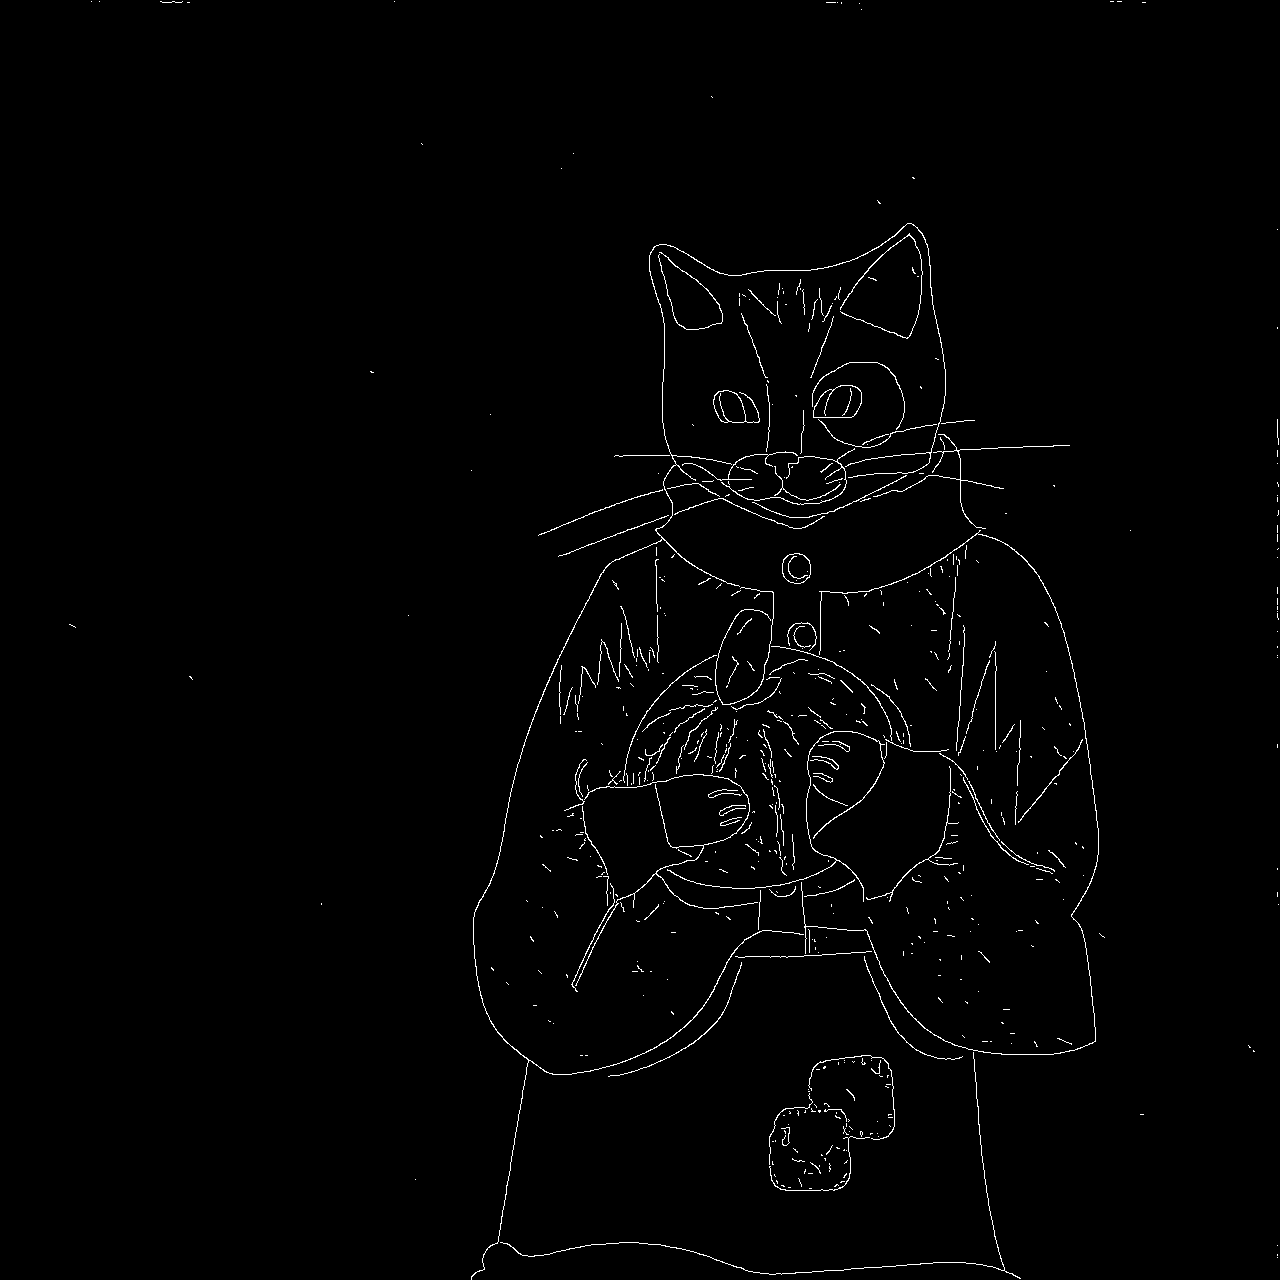
\includegraphics[width=\linewidth]{edges.png}
    \caption{Detected edges: ridge-NMS of $\hat B$, thresholded at $t_{\mathrm{edge}} = 1/2$.}
    \label{fig:edges}
  \end{subfigure}
  \caption{Qualitative result on one natural image from outside the BRIND splits, with the released model. Left: input. Right: HaCI edge map at inference.}
  \label{fig:example}
\end{figure}

% ─────────────────────────────────────────────────────────────────────
\section{Parameter Inventory}\label{sec:params}

The pipeline has $161$ learnable parameters (\cref{tab:learned-params}) and a handful of fixed structural constants (\cref{tab:fixed-params}). The renderer's correction MLP accounts for $124$ of the learned parameters; everything else is interpretable scalars (gains, half-saturation constants, anisotropy widths) or small monotone-parameterised filter taps.

\begin{table}[h]
\centering
\caption{Fixed structural and numerical constants.}
\label{tab:fixed-params}
\renewcommand{\arraystretch}{1.15}
\begin{tabular}{llc}
\toprule
Block & Symbol & Value\\
\midrule
L0 luminance half-saturation & $\eta_{\mathrm{lum}}$ & $0.01$ \\
L0 chrominance half-saturation & $\eta_{\mathrm{chr}}$ & $0.01$ \\
L0 notch half-width & $H_N$ & $4$ \\
L0 gain-control pool radius & $r_Q$ & $16$\,px \\
L1 cell size & $P$ & $5$\,px \\
L1 cell overlap & $O$ & $3$\,px (stride $D = 2$) \\
L1 border-cell fraction & --- & $0.2$ \\
L1/Seed orientation bins & $K$ & $8$ \\
Seed association-field radius & $r_f$ & $5$ cells \\
Seed surround radius & $r_S$ & $10$ cells \\
Seed flank radius & $r_{\mathrm{fl}}$ & $5$ cells \\
Seed flank normal tuning & $\kappa_{\mathrm{fl}}$ & $2.0$ \\
Seed flank exclusion (Chebyshev) & $r_{\mathrm{ex}}$ & $\lceil P/D \rceil - 1 = 2$ cells \\
Seed STE temperature & $\tau$ & $0.1$ \\
Renderer deposit half-width & $H_w$ & $\lceil 2 D \rceil = 4$\,px \\
Inference edge threshold & $t_{\mathrm{edge}}$ & $0.5$ \\
\bottomrule
\end{tabular}
\end{table}

\begin{table}[htbp]
\centering
\caption{Learned parameters. Positive scalars are reparameterised through $\softplus$ unless noted: $\omega_n$ and $d$ use a sigmoid, $\sigma_f$ and $\sigma_{\mathrm{fl}}$ are $1 + \softplus(\cdot)$, and $\sigma_S$ is clamped below at $0.3$. Angles are unbounded.}
\label{tab:learned-params}
\renewcommand{\arraystretch}{1.15}
\setlength{\tabcolsep}{3.5pt}
\begin{tabular}{llcr}
\toprule
Block & Symbol(s) & Init & \#params \\
\midrule
L0 metric gains & $w_\ell, s_1, s_2$ & $1.0$ & 3 \\
L0 chrominance angle & $\theta_{\mathrm{chr}}$ & $0$ & 1 \\
L0 notch & $\omega_n, \sigma_n, d$ & $1/8, 1/32, 0.8$ & 3 \\
L0 gain-control pool & $\lambda_0, \sigma_r$ & $10^{-5}, 2.0$ & 2 \\
\midrule
\multicolumn{3}{l}{\textbf{L0 subtotal}} & $\bm{9}$ \\
\midrule
Seed von~Mises concentration & $\kappa_{\mathrm{vm}}$ & $2.0$ & 1 \\
Seed NR half-saturation & $\eta_z$ & $10.0$ & 1 \\
Seed channel gain & $\beta_{\mathrm{seed}}$ & $0.5$ & 1 \\
Seed association gain & $\beta_{\mathrm{assoc}}$ & $0.5$ & 1 \\
Seed gap-bridge gain & $\beta_{\mathrm{gap}}$ & $0.5$ & 1 \\
Seed readout half-saturation & $\eta_r$ & $0.3$ & 1 \\
Seed surround weight & $\lambda$ & $0.5$ & 1 \\
Seed association reach & $\sigma_f$ ($\geq 1$) & $2.0$ & 1 \\
Seed association direction tuning & $\kappa_a$ & $8.0$ & 1 \\
Seed curvature tolerance & $\sigma_\kappa$ & $0.01$ & 1 \\
Seed surround width & $\sigma_S$ ($\geq 0.3$) & $1.0$ & 1 \\
Seed flank weight & $\lambda_{\mathrm{fl}}$ & $0.01$ & 1 \\
Seed flank reach & $\sigma_{\mathrm{fl}}$ ($\geq 1$) & $2.0$ & 1 \\
\midrule
\multicolumn{3}{l}{\textbf{Seed subtotal}} & $\bm{13}$ \\
\midrule
Renderer correction MLP $5\to 12\to 4$ & $\Phi$ & near-zero output & 124 \\
Renderer correction bounds & $\kappa_{\max}, \xi_{\max}, \delta_{n,\max}, \alpha_{\mathrm{range}}$ & $0.1, 1, 1, 0.5$ & 4 \\
Renderer gate temperature & $T_{\mathrm{gate}}$ & $0.08$ & 1 \\
Renderer radial filter & $\{\nu_m\}_{m=0}^{H_w}$ & Hann $\omega_c=0.5$ & 5 \\
Renderer longitudinal filter & $\{\zeta_j\}_{j=1}^{H_w}, h_0$ & Gaussian $\sigma_{\parallel,0}=2$ & 5 \\
\midrule
\multicolumn{3}{l}{\textbf{Renderer subtotal}} & $\bm{139}$ \\
\midrule
\multicolumn{3}{l}{\textbf{Total}} & $\bm{161}$ \\
\bottomrule
\end{tabular}
\end{table}

% ─────────────────────────────────────────────────────────────────────
\section{Discussion}\label{sec:discussion}

HaCI compresses a classical contour-integration computation into a fully differentiable graph of $161$ scalars. The choice of what to expose to data and what to fix is rooted in the strict interpretation of cortical mechanisms. The renderer's $5 \to 12 \to 4$ correction head is the only learned component that is neither a named scalar nor a constrained filter; it is there to handle off-anchor edges, sub-pixel curvature and bin selectivity at junctions. With its output held at zero ($\kappa = \xi = \delta_n = 0$, $\alpha = 1$) the renderer reduces to a straight-stroke depositor; how much the head adds over that is not measured in this report. The kernels $h_{\perp}, h_{\parallel}$ are parameterised so that every point in parameter space is a valid windowed-ramp radial filter and a positive monotone-decay longitudinal profile, respectively. This keeps the synthesis path interpretable as a ramp-filtered stroke deposit, while leaving the kernel shape open to gradient descent against the boundary objective.

This report fixes the equations and reports results on BRIND (\cref{sec:results}); ablations and comparison against deep baselines~\cite{xie2015hed,liu2017rcf,he2019bdcn,pu2022edter,soria2023dexined,ye2024diffusionedge} are deferred to a forthcoming full paper.

\section*{Code availability}
The reference implementation is available at \url{https://github.com/RenderBear/haci}.

% =====================================================================
\appendix

\section{Per-bin Renderer Features}\label{app:feats}

The five features in \cref{eq:feats} are computed from the 3$\times$3 neighbourhood $\mathcal{N}_3(c)$ of cell $c$ (with $\delta \in \mathcal{N}_3 \setminus \{0\}$) as follows. Let $t_k(\delta) = \delta_y \cos\bar\theta_k + \delta_x \sin\bar\theta_k$ and $n_k(\delta) = -\delta_y \sin\bar\theta_k + \delta_x \cos\bar\theta_k$ be the tangent and normal projections of the offset in bin $k$, and $\mathrm{pos}_t^{(k)}(\delta) = t_k(\delta)^2/\norm{\delta}^2$. Then
\begin{align}
  \mu^{(k)}_{\mathrm{coll}}(c) &= \frac{\sum_\delta \rho_{\mathrm{out}}^{(k)}(c+\delta)\,\mathrm{pos}_t^{(k)}(\delta)}
                                       {\sum_\delta \mathrm{pos}_t^{(k)}(\delta) + \varepsilon'}, \\
  \mu^{(k)}_t(c) &= \frac{\sum_\delta \rho_{\mathrm{out}}^{(k)}(c+\delta)\, t_k(\delta)}
                          {\sum_\delta \rho_{\mathrm{out}}^{(k)}(c+\delta)\, \abs{t_k(\delta)} + \varepsilon'}, \\
  \mu^{(k)}_n(c) &= \frac{\sum_\delta \rho_{\mathrm{out}}^{(k)}(c+\delta)\, n_k(\delta)}
                          {\sum_\delta \rho_{\mathrm{out}}^{(k)}(c+\delta)\, \abs{n_k(\delta)} + \varepsilon'},
\end{align}
with a soft floor $\varepsilon' = 5\times 10^{-2}$ on the denominator. $\mu^{(k)}_{\mathrm{coll}}$ summarises collinear support along the bin tangent; $\mu^{(k)}_t \in [-1, 1]$ is a signed tangent asymmetry that signals where, along the tangent, the local mass is concentrated, and is meant as the cue for the tangent shift $\xi$; $\mu^{(k)}_n \in [-1, 1]$ is the analogous normal asymmetry, meant as the cue for $\delta_n$. Nothing enforces this pairing: $\Phi$ is a dense MLP, so every feature reaches all four outputs.

\section{Renderer parameter count}\label{app:render-count}

The correction MLP has $5 \cdot 12 + 12 = 72$ parameters in the input layer and $12 \cdot 4 + 4 = 52$ in the output layer, for $124$ total. The kernel radial logits $\{\nu_m\}$ have $H_w + 1 = 5$ parameters; the longitudinal logits $\{\zeta_j\}$ have $H_w = 4$ parameters; the longitudinal peak adds $1$. The four correction bounds $(\kappa_{\max}, \xi_{\max}, \delta_{n,\max}, \alpha_{\mathrm{range}})$ and the gate temperature $T_{\mathrm{gate}}$ contribute $5$ further scalars. Total: $124 + 4 + 1 + 5 + 4 + 1 = 139$.

% =====================================================================
\begin{thebibliography}{99}

\bibitem{naka1966srod}
K.~I.~Naka, W.~A.~H.~Rushton.
\newblock S-potentials from colour units in the retina of fish (Cyprinidae).
\newblock \emph{Journal of Physiology}, 185(3):536--555, 1966.

\bibitem{hubel1962orientation}
D.~H.~Hubel, T.~N.~Wiesel.
\newblock Receptive fields, binocular interaction and functional architecture in the cat's visual cortex.
\newblock \emph{Journal of Physiology}, 160(1):106--154, 1962.

\bibitem{heeger1992normalisation}
D.~J.~Heeger.
\newblock Normalization of cell responses in cat striate cortex.
\newblock \emph{Visual Neuroscience}, 9(2):181--197, 1992.

\bibitem{cavanaugh2002surround}
J.~R.~Cavanaugh, W.~Bair, J.~A.~Movshon.
\newblock Nature and interaction of signals from the receptive field center and surround in macaque V1 neurons.
\newblock \emph{Journal of Neurophysiology}, 88(5):2530--2546, 2002.

\bibitem{kapadia1995dynamics}
M.~K.~Kapadia, M.~Ito, C.~D.~Gilbert, G.~Westheimer.
\newblock Improvement in visual sensitivity by changes in local context: parallel studies in human observers and in V1 of alert monkeys.
\newblock \emph{Neuron}, 15(4):843--856, 1995.

\bibitem{field1993contour}
D.~J.~Field, A.~Hayes, R.~F.~Hess.
\newblock Contour integration by the human visual system: Evidence for a local ``association field''.
\newblock \emph{Vision Research}, 33(2):173--193, 1993.

\bibitem{zhou2000border}
H.~Zhou, H.~S.~Friedman, R.~von~der~Heydt.
\newblock Coding of border ownership in monkey visual cortex.
\newblock \emph{Journal of Neuroscience}, 20(17):6594--6611, 2000.

\bibitem{parent1989trace}
P.~Parent, S.~W.~Zucker.
\newblock Trace inference, curvature consistency, and curve detection.
\newblock \emph{IEEE Transactions on Pattern Analysis and Machine Intelligence}, 11(8):823--839, 1989.

\bibitem{pu2021rindnet}
M.~Pu, Y.~Huang, Q.~Guan, H.~Ling.
\newblock RINDNet: Edge Detection for Discontinuity in Reflectance, Illumination, Normal and Depth.
\newblock In \emph{IEEE/CVF International Conference on Computer Vision (ICCV)}, 2021.

\bibitem{canny1986computational}
J.~Canny.
\newblock A computational approach to edge detection.
\newblock \emph{IEEE Transactions on Pattern Analysis and Machine Intelligence}, 8(6):679--698, 1986.

\bibitem{arbelaez2011gpb}
P.~Arbeláez, M.~Maire, C.~Fowlkes, J.~Malik.
\newblock Contour detection and hierarchical image segmentation.
\newblock \emph{IEEE Transactions on Pattern Analysis and Machine Intelligence}, 33(5):898--916, 2011.

\bibitem{kak2001ct}
A.~C.~Kak, M.~Slaney.
\newblock \emph{Principles of Computerized Tomographic Imaging}.
\newblock SIAM Classics in Applied Mathematics 33, 2001.

\bibitem{kingma2014adam}
D.~P.~Kingma, J.~Ba.
\newblock Adam: A method for stochastic optimization.
\newblock In \emph{International Conference on Learning Representations (ICLR)}, 2015.

\bibitem{xie2015hed}
S.~Xie, Z.~Tu.
\newblock Holistically-Nested Edge Detection.
\newblock In \emph{IEEE International Conference on Computer Vision (ICCV)}, 2015.

\bibitem{liu2017rcf}
Y.~Liu, M.-M.~Cheng, X.~Hu, K.~Wang, X.~Bai.
\newblock Richer Convolutional Features for Edge Detection.
\newblock In \emph{IEEE Conference on Computer Vision and Pattern Recognition (CVPR)}, 2017.

\bibitem{he2019bdcn}
J.~He, S.~Zhang, M.~Yang, Y.~Shan, T.~Huang.
\newblock BDCN: Bi-Directional Cascade Network for Perceptual Edge Detection.
\newblock In \emph{IEEE Conference on Computer Vision and Pattern Recognition (CVPR)}, 2019.

\bibitem{pu2022edter}
M.~Pu, Y.~Huang, Y.~Liu, Q.~Guan, H.~Ling.
\newblock EDTER: Edge Detection with Transformer.
\newblock In \emph{IEEE Conference on Computer Vision and Pattern Recognition (CVPR)}, 2022.

\bibitem{soria2023dexined}
X.~Soria, A.~Sappa, P.~Humanante, A.~Akbarinia.
\newblock Dense Extreme Inception Network for Edge Detection.
\newblock \emph{Pattern Recognition}, 139:109461, 2023.

\bibitem{ye2024diffusionedge}
Y.~Ye, K.~Xu, Y.~Huang, R.~Yi, Z.~Cai.
\newblock DiffusionEdge: Diffusion Probabilistic Model for Crisp Edge Detection.
\newblock In \emph{AAAI Conference on Artificial Intelligence}, 2024.

\end{thebibliography}

\end{document}